% Made up for the tikra gallery: a parabola in vertex form. In the playground, drag its vertex;
% the opening a is a number of its own.
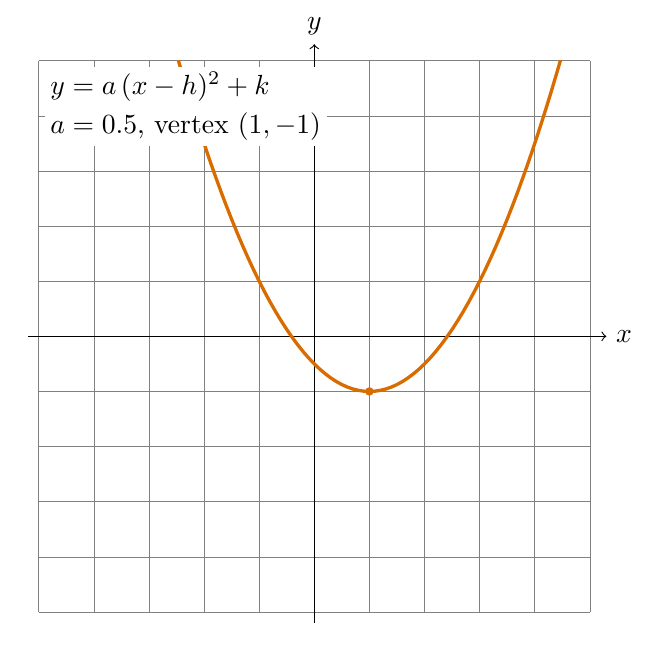
\begin{tikzpicture}[scale=0.7]
  \def\a{0.5}  % opening, -2..2
  \def\h{1}    % x of the vertex, -3..3:0.1
  \def\k{-1}   % y of the vertex, -3..3:0.1
  \useasboundingbox (-5.2,-5.2) rectangle (5.6,5.6);
  \draw[help lines] (-5,-5) grid (5,5);
  \draw[->] (-5.2,0) -- (5.3,0) node[right] {$x$};
  \draw[->] (0,-5.2) -- (0,5.3) node[above] {$y$};
  \begin{scope}
    \clip (-5,-5) rectangle (5,5);
    \draw[very thick, orange!85!black, domain=-5:5, samples=101] plot (\x, {\a*(\x-\h)^2 + \k});
  \end{scope}
  \coordinate (vertex) at (\h,\k);
  \fill[orange!85!black] (vertex) circle (2.2pt);
  \node[fill=white, inner sep=2pt, anchor=north west, align=left] at (-4.9,4.9) {$y = a\,(x - h)^2 + k$\\[2pt]
    $a = \pgfmathprintnumber{\a}$, vertex $(\pgfmathprintnumber{\h}, \pgfmathprintnumber{\k})$};
\end{tikzpicture}
